\documentclass[11pt,a4paper]{article}
\usepackage[margin=0.8in]{geometry}
\usepackage[T1]{fontenc}
\usepackage[utf8]{inputenc}
\usepackage{lmodern}
\usepackage{amsmath,amssymb}
\usepackage{graphicx}
\usepackage{caption}
\usepackage{booktabs}
\usepackage{longtable}
\usepackage{tabularx}
\usepackage{enumitem}
\usepackage{hyperref}
\usepackage{xcolor}

% Custom Colors for a professional look
\definecolor{aybu_blue}{RGB}{31, 73, 125}
\definecolor{section_gray}{RGB}{242, 242, 242}

\hypersetup{
    colorlinks=true,
    linkcolor=aybu_blue,
    urlcolor=blue
}

\graphicspath{{./diagrams_aybustore/}}

\title{\LARGE \textbf{AYBUStore: Intelligent Campus E-Commerce Ecosystem}\\[0.5em] \large Supplementary Technical Report for TÜBİTAK 1001 Proposal}
\author{Utkan Dindaroğlu, Seyfullah Gülyazı, Süleyman Fatih Sert, Ahmet Selim Yılmaz, Muhammed Yıldız}
\date{\today}

\begin{document}

\maketitle

\begin{abstract}
This report details the technical architecture, methodology, and requirement specifications for AYBUStore, a smart e-commerce platform developed for Ankara Yıldırım Beyazıt University. Utilizing a modern stack of Next.js 14 and Firebase, the project integrates AI-driven personalization and real-time inventory management to solve physical campus commerce inefficiencies.
\end{abstract}

\section{Introduction \& Problem Definition}
The AYBUStore project addresses the lack of a centralized digital ecosystem for university-branded merchandise and department-specific materials. Existing solutions fail to provide real-time stock transparency, personalized apparel preview, or AI-integrated shopping assistance.

\section{System Architecture}
We adopt a \textbf{Component-Based Architecture} using Next.js App Router for optimal performance and SEO. The backend is powered by Firebase, providing a serverless real-time database and secure authentication.

\subsection{Use Case Analysis}
The following diagram illustrates the interactions between students, staff, and administrators within the ecosystem.

\begin{center}
    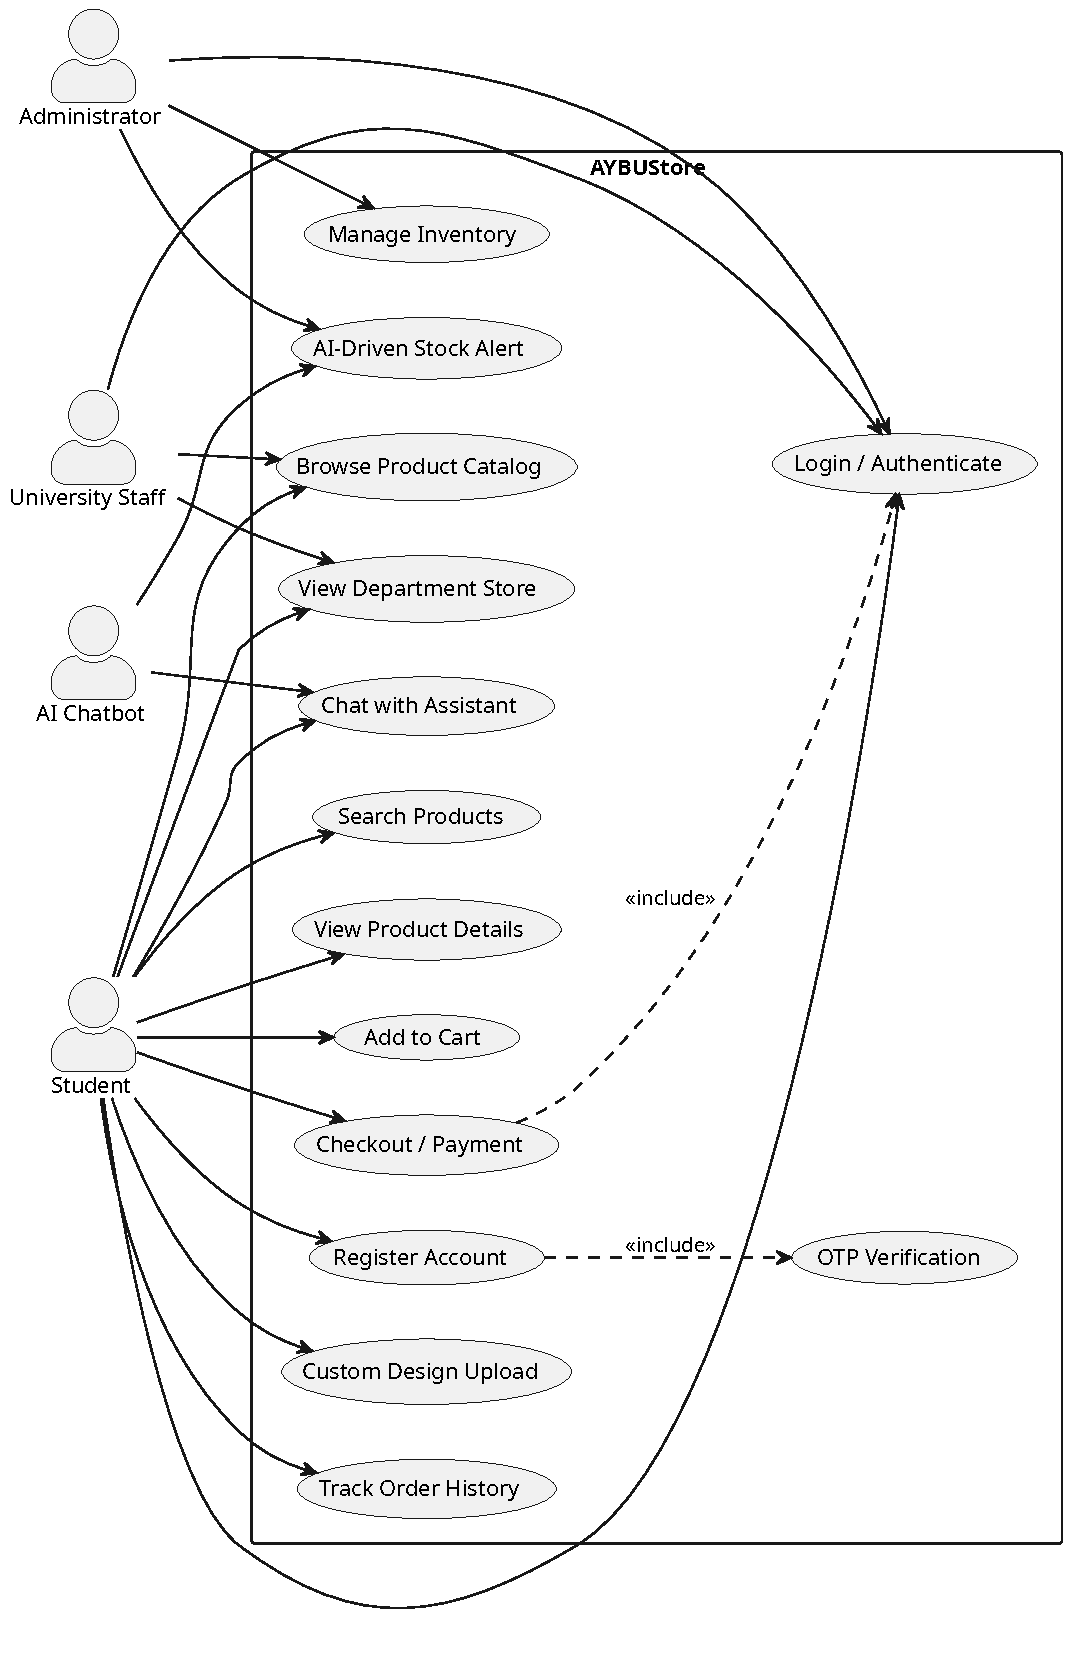
\includegraphics[width=0.8\textwidth]{use_case_diagram}
    \captionof{figure}{AYBUStore Use Case Diagram (Vector)}
\end{center}

\subsection{Domain Modeling}
The system's data structure is designed with modularity in mind, ensuring scalability as new faculties are added.

\begin{center}
    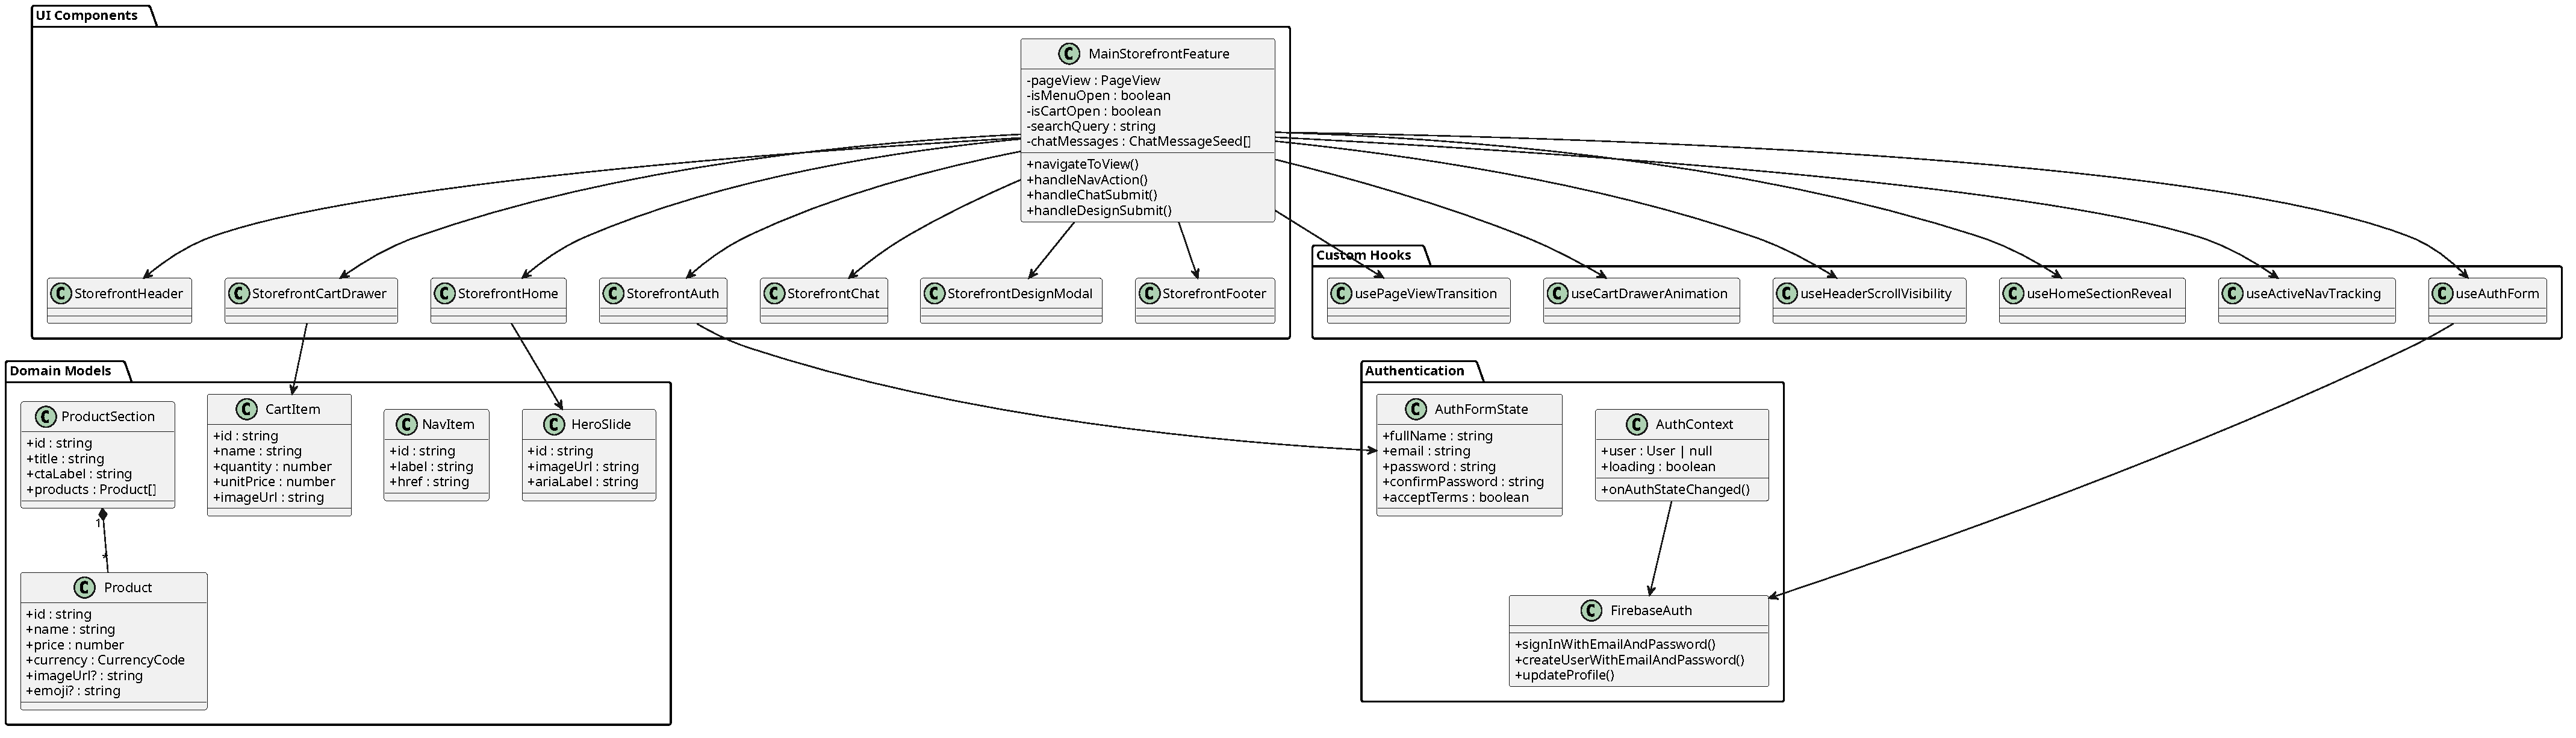
\includegraphics[width=0.9\textwidth]{class_diagram}
    \captionof{figure}{System Domain Class Diagram}
\end{center}

\section{Core Processes}
\subsection{Authentication \& OTP Flow}
Security is managed via a multi-stage authentication process, verified by a 6-digit one-time password (OTP) sent to university emails.

\begin{center}
    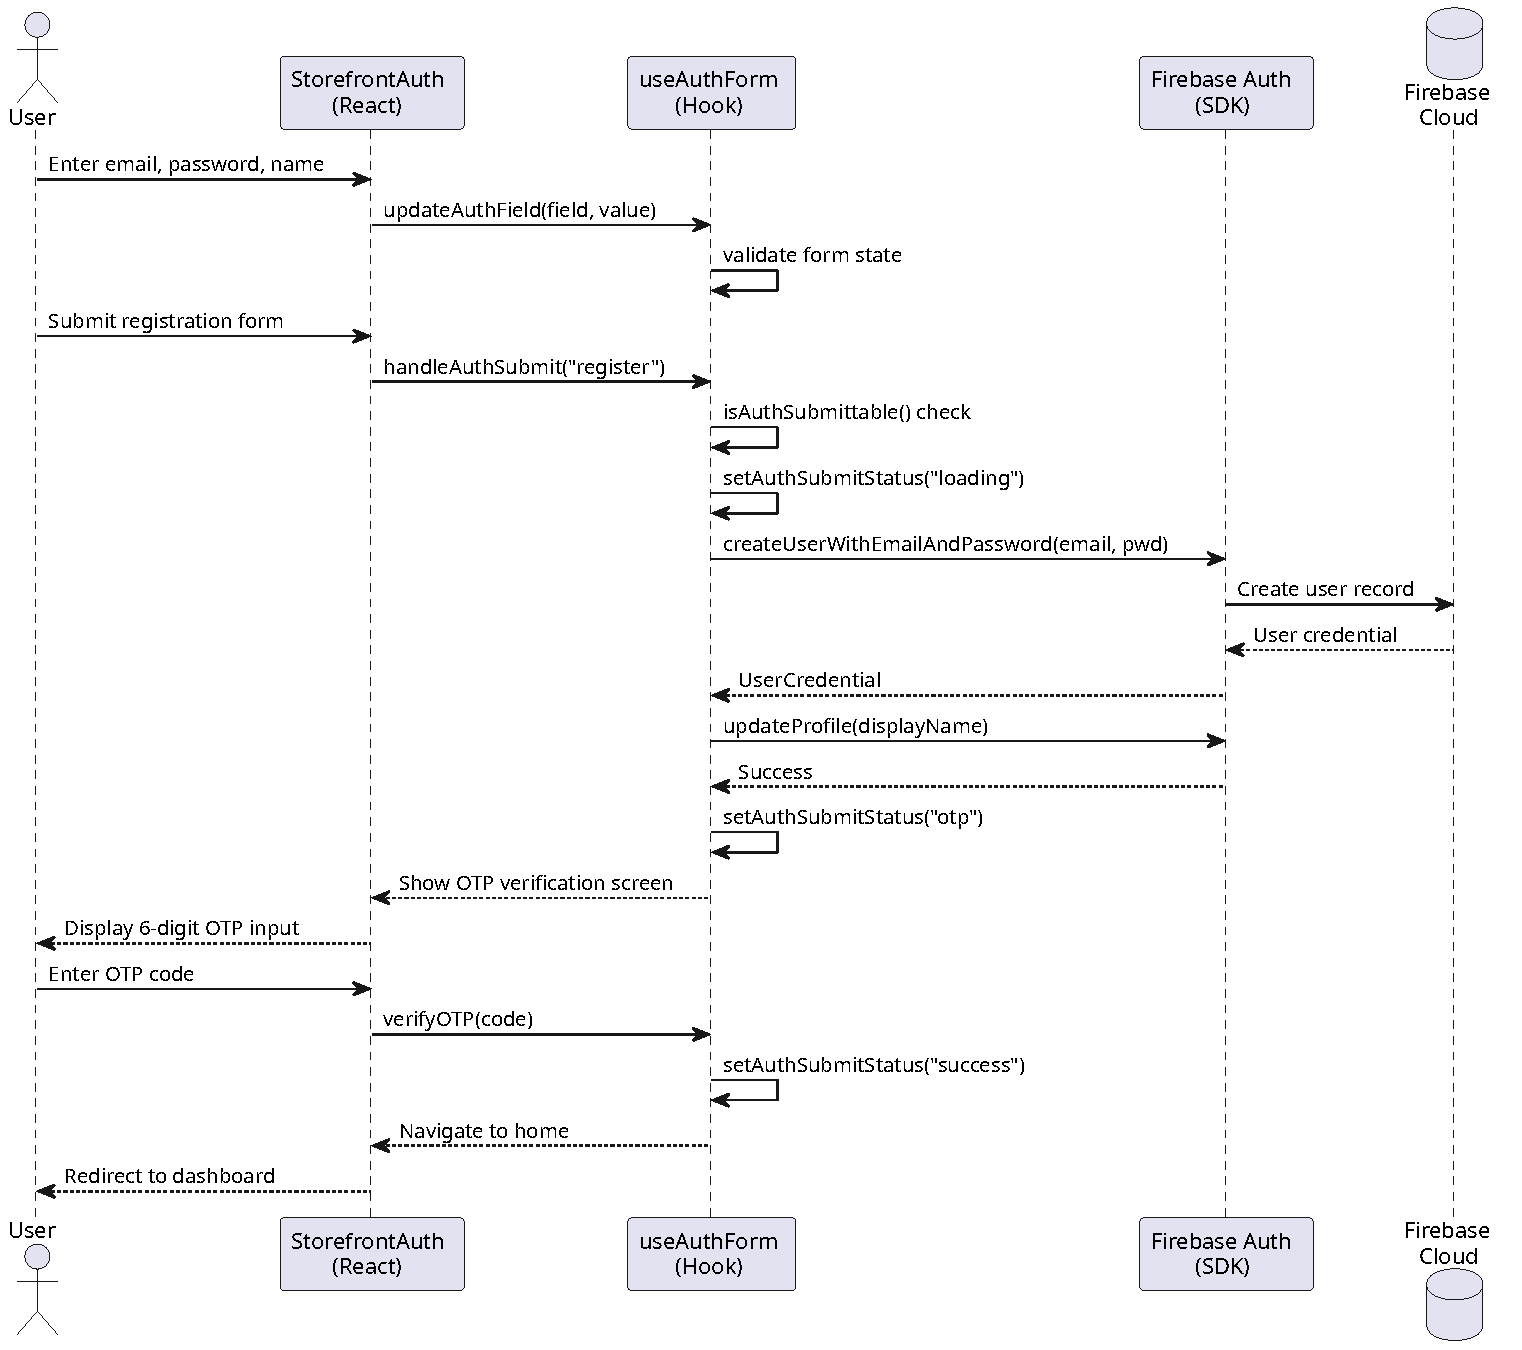
\includegraphics[width=0.8\textwidth]{sequence_auth}
    \captionof{figure}{Registration and Security Verification Sequence}
\end{center}

\subsection{AI Personalization}
The AI Shopping Assistant utilizes LLM-based intent analysis to provide context-aware product recommendations.

\begin{center}
    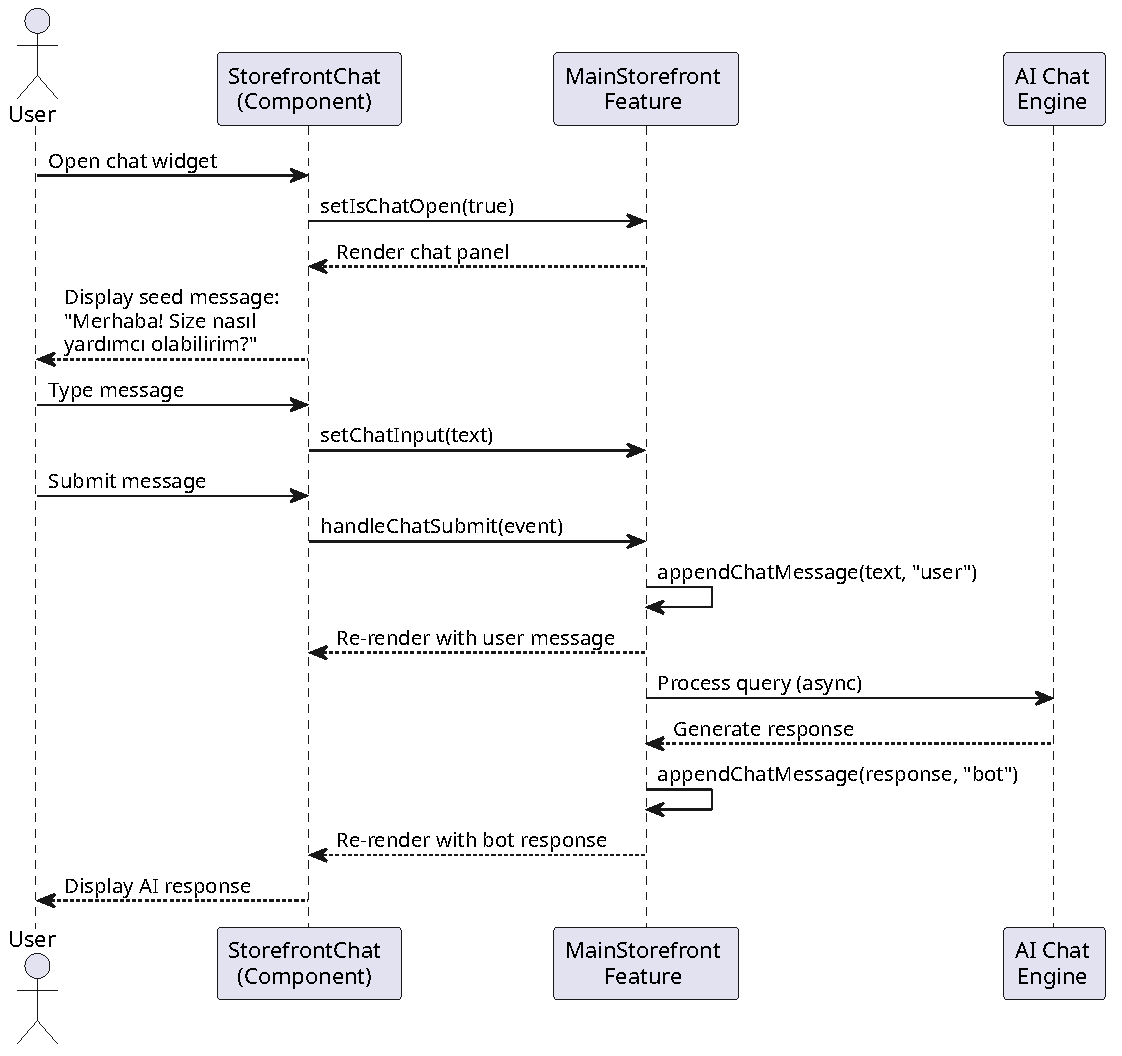
\includegraphics[width=0.8\textwidth]{sequence_chat}
    \captionof{figure}{AI-Driven Assistant Interaction Flow}
\end{center}

\section{Operational Design}
\subsection{Shopping Lifecycle}
The activity flow below describes the transition from browsing to custom design and final checkout.

\begin{center}
    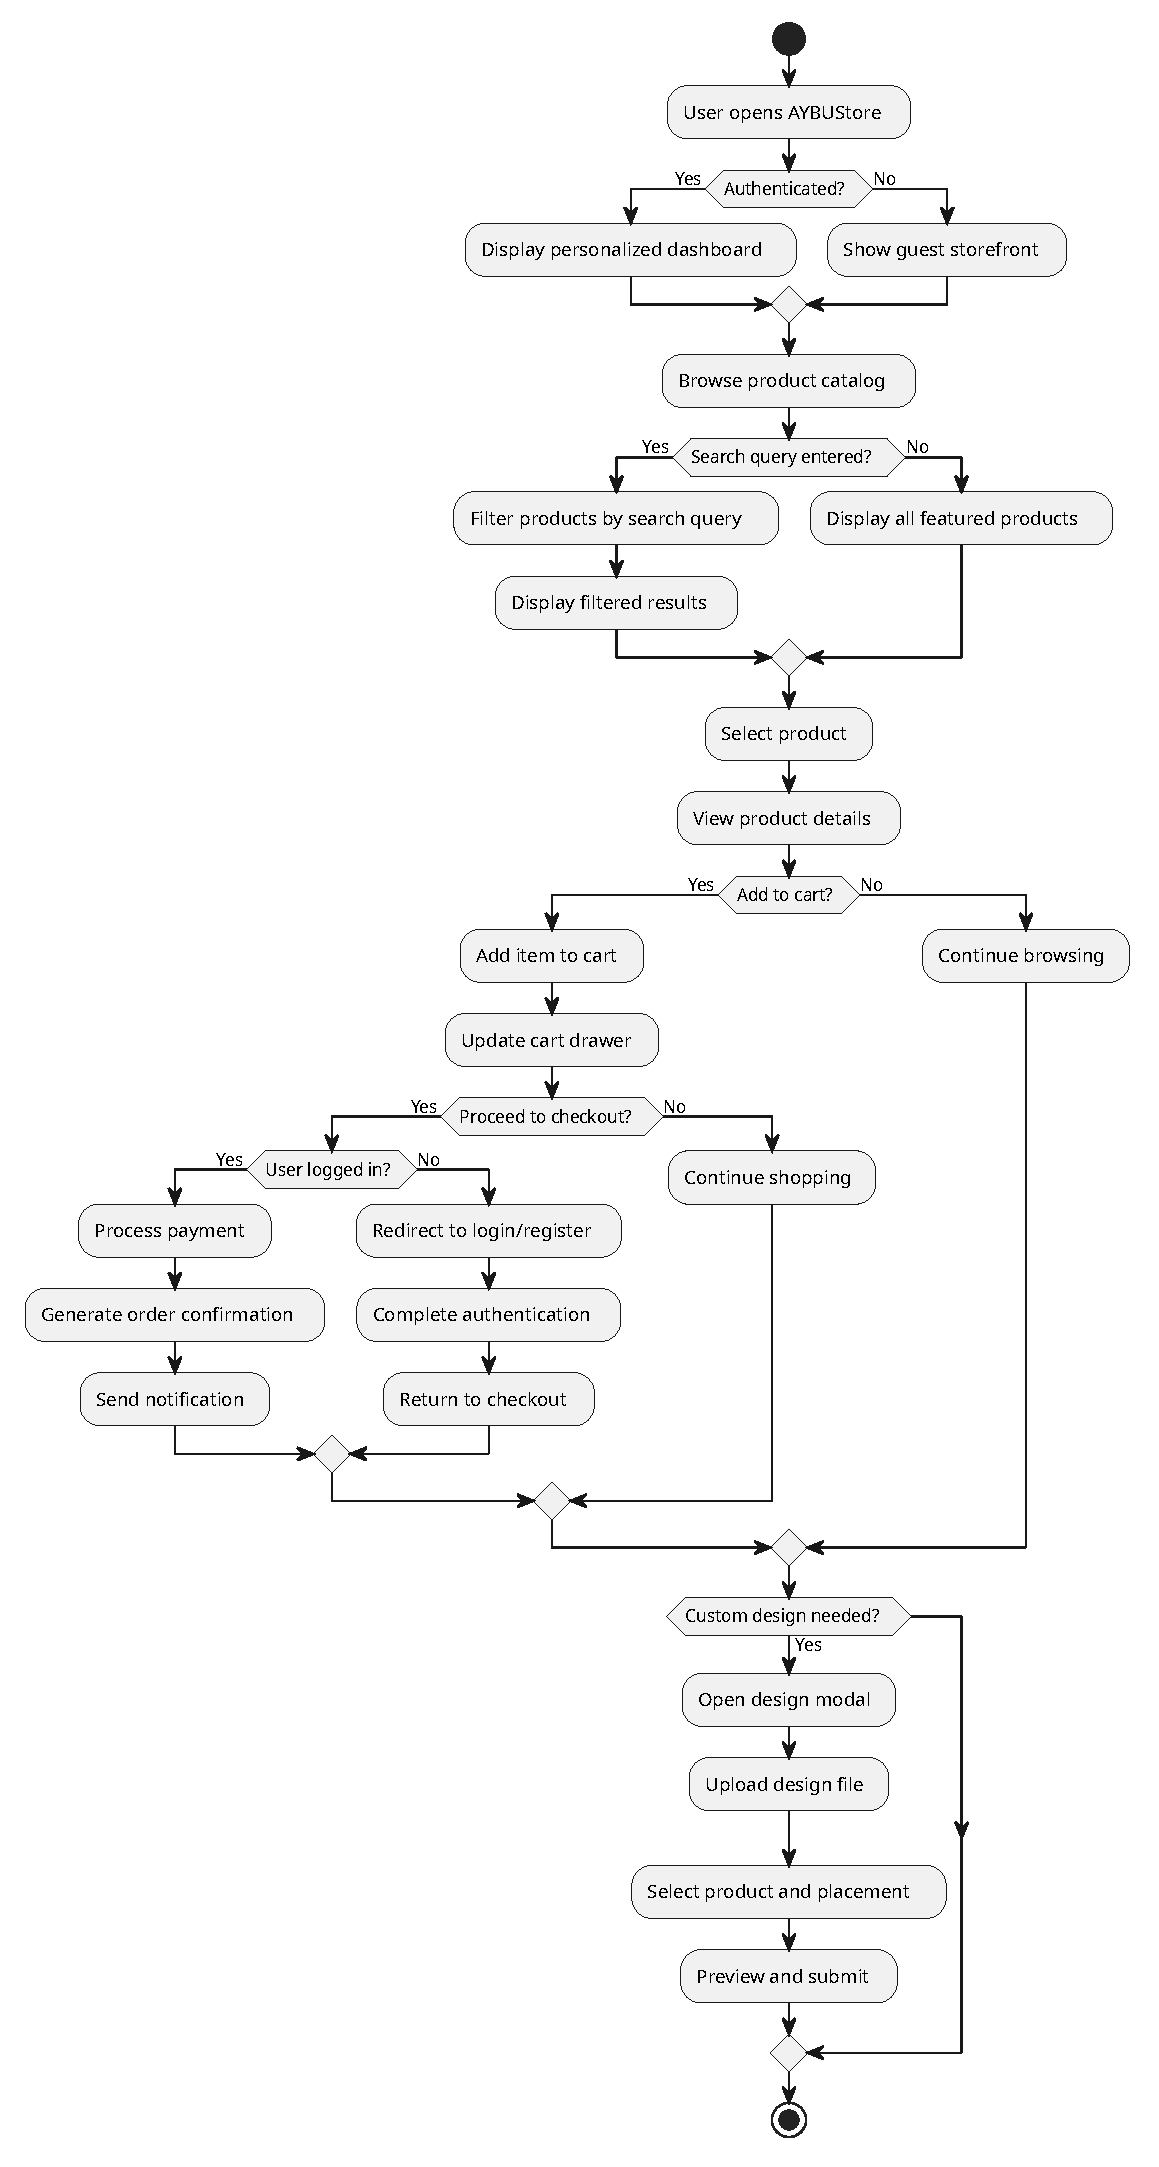
\includegraphics[width=0.8\textwidth]{activity_diagram}
    \captionof{figure}{User Activity Lifecycle Diagram}
\end{center}

\section{Implementation Plan}
The project follows an \textbf{Agile/Scrum} framework divided into four primary sprints:
\begin{enumerate}
    \item \textbf{Sprint 1:} Core Infrastructure \& Design System.
    \item \textbf{Sprint 2:} Auth, Product Catalog \& Cart Engine.
    \item \textbf{Sprint 3:} AI Integration \& Custom Design Module.
    \item \textbf{Sprint 4:} Performance Optimization \& User Acceptance Testing.
\end{enumerate}

\section{Conclusion}
AYBUStore provides a scalable and intelligent solution for campus commerce, leveraging modern web technologies to enhance the university's digital brand.

\end{document}
